\newpage
\section{Logistic Regression Basics}
\label{sec:logistic_regression_basics}

Dieses Kapitel beschreibt die fundamentalen Aspekte (prüfungsrelevanter Teil) der logistischen Regression. Die logistic regression ist ein linearer suppervised Klassifikationsalgorithmus. Genauer genommen einen \textbf{binären} Klassifikationsalgorithmus. \\


\subsection{Logistic Regression vs Adaline}

Die grundlegende Architektur von logistic regression ist sehr ähnlich wie bei Adaline. Der \textbf{Hauptunterschied} liegt bei der Aktivierungsfunktion. Die logistic regression verwendet die sogenannte \textbf{Sigmoid} Funktion.

Für Adaline haben wir lediglich die Identitätsfunktion verwendet.


\begin{figure}[h!]
	\includegraphics[scale=0.5]{figures/logistic_regression_vs_adaline}
	\caption{Logistic Regression vs Adaline}
	\label{fig:lr_vs_adaline}
\end{figure}


\newpage
\subsection{Sigmoid Funktion}

Die Sigmoid Funktion nimmt einen Input und transformiert diesen in ein Bereich [0,1].

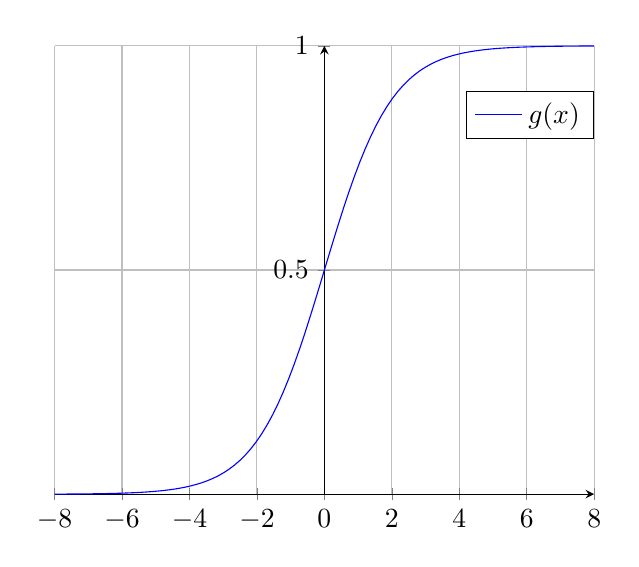
\begin{tikzpicture}[declare function={sigma(\x)=1/(1+exp(-\x));}]
\begin{axis}%
[
    grid=major,     
    xmin=-8,
    xmax=8,
    axis x line=bottom,
    ytick={0,.5,1},
    ymax=1,
    axis y line=middle,
    samples=100,
    domain=-8:8,
    legend style={at={(1,0.9)}}     
]
    \addplot[blue,mark=none]   (x,{sigma(x)});
    \legend{$g(x)$}
\end{axis}
\end{tikzpicture}


$$ \phi(z) = \frac{1}{1 + e^{-z}} $$

Der Wert von $\phi(z)$ kann auch als \textbf{Wahrscheinlichkeit} interpretiert werden, das ein gewisses Sample zu einer bestimmten Klasse gehört.


$$ \phi(z) = \frac{1}{1 + e^{-z}} = P(y=1 | x;w) $$
Hierbei steht $y=1$ für die binäre Klasse 1.
Somit gilt auch der Zusammenhang zur anderen Klasse 0:
$$ P(y=0|x;w) = 1 - P(y=1|x;w)$$


\subsection{Vorteile logistic regression}

\begin{itemize}
	\item Output der Sigmoid kann als Wahrscheinlichkeit interpretiert werden. Dies gibt uns Informationen über die \textbf{Gewissheit} des Models.
	\item Da logistic regression ein \textbf{lineares Model} ist, ist es einfach zu interpretieren, updaten und ist skalierbar.
\end{itemize}

Diese Vorteile machen die logistische Regression zu einer zuverlässige und sinnvolle Wahl für viele Klassifizierungsprobleme.




